\chapter{定理证明的可视化}\label{chapt:visulization}
在数理逻辑领域,一个逻辑公式的形式化证明通常被表示成一个公式序列,其中这个公式序列中的每个公式既可以是公理,也可以是之前公式的逻辑推导结论。一种更加自然的表示公式的形式化证明的方式是将证明表示成一棵树,其中这颗树的每一个节点都用一个公式标记,而该节点的子节点则标记为相应公式的逻辑前提。如今,随着计算机定理证明工具的应用,逻辑公式的形式化证明树可由计算机以自动或者半自动(需要人工干预)的方式生成。然而,目前定理证明工具的输出都是文本格式的,这就使得当证明树的结构较复杂或者节点较多的时候不容易使人理解。同样的问题也出现在模型检测领域,当Kripke模型的结构较复杂的时候,文本格式的输出通常无法直观地展示由模型检测工具生成的反例。
另外,在上一章中我们提到,\sctlprov{}在验证Kripke模型的性质时,相比于传统的模型检测工具,能生成更丰富的验证结果。\couic{而且,在传统的模型检测工具和定理证明工具中,验证的结果通常是以文本形式输出的,而文本形式的输出通常无法清晰地表达对于结构复杂的Kripke模型的状态搜索,也无法完整展现模态词嵌套的公式的证明树。}为了能将\sctlprov{}的证明输出结果以及证明过程得以清晰并完整地展现出来,在本章我们介绍\tool{VMDV}\footnote{\url{https://github.com/terminatorlxj/VMDV}}(Visualization for Modeling, Demonstration and Verification)。

\tool{VMDV}是一个将证明树及其他数据结构(比如Kripke模型)在3D空间内进行动态可视化布局和显示的工具。相比于其他的证明可视化工具,\tool{VMDV}具有四个特点:
\begin{enumerate}
	\item 目前大多数的证明可视化工具\cite{byrnes2009visualizing,LibalRR14,sakurai2011mikibeta,steel2005visualising}都使用2D图形来完成证明树的绘制,并且可以用不同的颜色来区分证明树中不同的分支或节点。不同于这些工具,\tool{VMDV}是在3D空间中实现证明树的绘制,除了具备2D图形相比文本格式更直观的优点之外,3D空间相比2D空间可以容纳更多的节点和更复杂的图形结构,从而在展示大型证明树时更有优势。
	\item 另一方面,除了\tool{VMDV}之外,目前也有其他可在3D空间内实现证明树绘制的工具\cite{Farmer200939,bajaj2003interactive}。然而,目前的3D证明可视化工具的布局算法是比较原始的,当在这些工具中展示较多的节点时,所有的节点往往按照一个或若干个既定的方向做延伸状排列,这种布局方式使得3D图形的展示既不美观,又降低了空间利用率。不同于这些工具,\tool{VMDV}利用动态布局算法,将所有的节点看作是相互之间具有斥力的物体,而连接节点之间的边则可看作是具有引力的弹簧,通过每个节点所受的引力和斥力来随时更新节点在3D空间内的位置,并在整个布局过程中随时更新节点间的引力和斥力,直到所有节点的受力达到平衡状态。整个证明树就可看作一个自适应的物理系统,由此得出的节点布局更自然美观,也能充分填充3D空间。
	\item 在传统的具有人工干预的定理证明工具(比如Coq\footnote{\url{https://coq.inria.fr/}})中,证明树的节点通常随时被加入或者删除。\tool{VMDV}可实现证明树结构的动态更新的可视化。
	\item 不同于传统的证明可视化工具通常只针对于一种定理证明工具的输出的可视化,我们在\tool{VMDV}中定义了可与不同的定理证明工具的接口\footnote{\url{https://github.com/terminatorlxj/VMDV/blob/master/protocol.md}}。实现这个接口的定理证明工具或者其插件都可以利用\tool{VMDV}的功能来实现证明的可视化。
\end{enumerate}


\tool{VMDV}利用\textsf{OpenGL}的绘图接口来编写显示引擎,并用Java编程语言来实现布局算法与其他工具的数据通信。接下来,我们分别介绍\tool{VMDV}的相关技术细节及其应用。

\section{背景知识}
这一小节讲的是有关可视化的相关背景知识。
\subsection{OpenGL}\label{vmdv:opengl}
\textsf{OpenGL},全称Open Graphics Library,是一个跨编程语言并且跨平台的编程接口的标准。在计算机系统中,通常由显卡提供\textsf{OpenGL}的实现。一个典型的基于\textsf{OpenGL}的3D图形的显示过程为:首先,用户程序通过调用\textsf{OpenGL}的绘图\textsf{API}(Application Programming Interface)来定义一组要显示的图形的数据和命令,并将这些数据和命令存储在计算机的主内存(RAM)中;然后,计算机的中央处理器(CPU)会通过CPU时钟将这些数据和命令发送到显卡的显存(VRAM)中,并在图形处理器(GPU)的控制下完成图形的渲染;最后,图形渲染的结果会被存入帧缓冲区中,而帧缓冲区中的帧则最终被发送到计算机的显示器上,并显示出结果。

\subsection{信息可视化}
信息可视化是一个研究如何利用计算机图形学技术将数据中的抽象信息可视化的研究领域。抽象信息的可视化表达可以用来帮助人们揭示数据的隐匿模式,用来帮助更好地理解和发现数据中的规律。得益于计算机图形学理论的日益成熟以及计算机硬件的飞速发展,信息可视化系统能可视化越来越大的数据集以及越来越复杂的数据结构,并在许多行业中发挥着举足轻重的作用。比如,在知识管理领域,信息可视化系统可以用来研究不同学科领域知识之间的关系和演化\cite{ZHHW16};在城市交通系统的研究中,信息可视化系统可以将城市的公共交通工具的卫星定位数据进行可视化,以帮助人们研究和改善公共交通的效率\cite{FYL15}。

\section{\tool{VMDV}的实现}
这一小节讲的是\tool{VMDV}的架构,接口以及3D图形的自动布局算法。
\subsection{\tool{VMDV}的架构}
\begin{figure}[!h]
	\scriptsize
	%\vspace{2.5cm}
	\centering
	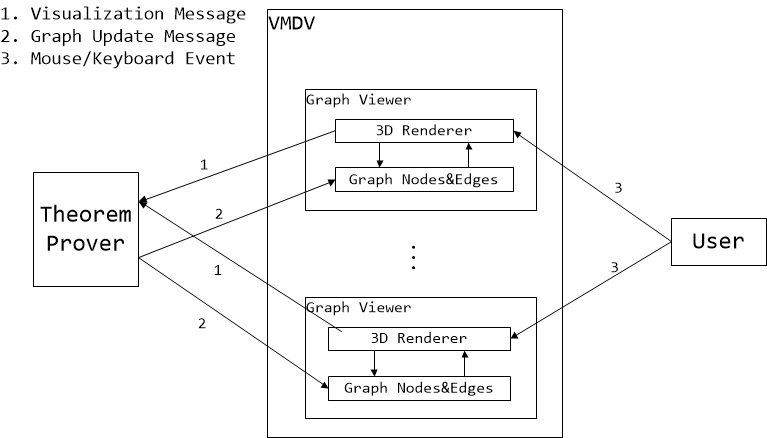
\includegraphics[width=12cm]{./Img/architecture.png}
	\caption{\textsf{VMDV}的架构}
	%\vspace{-10pt}
	\label{fig:architecture}
\end{figure}
如图\ref{fig:architecture}所示,\tool{VMDV}可同时在多个程序窗口中显示3D图形,在\tool{VMDV}中,每个程序窗口都分别包含一个3D渲染器和一个由多个点和边组成的图。3D渲染器的作用是读入图中的点和边的信息,然后根据布局算法确定点和边的位置,最后在3D空间中将图渲染出来。其中,图中的点和边可以通过接收定理证明器传递的消息来动态的添加、删除以及更改,同时3D渲染器对图的更改进行动态的显示,然后向定理证明器发送反馈消息。在3D渲染器工作的同时,\tool{VMDV}同样接收用户传递的交互消息(键盘或鼠标消息),并及时地在3D渲染器中做出反应。

可以看出,\tool{VMDV}同时可以接收两种消息:定理证明器传递过来的消息以及用户给定的消息。其中,定理证明器的消息是以\textsf{TCP}数据包的形式传输的。因此,定理证明器与\tool{VMDV}在网络上通过给定的通讯接口进行交互,而不一定在同一机器上甚至同一进程中。这种设计方式大大减少了\tool{VMDV}对特定的定理证明器的依赖。用户通过传递给\tool{VMDV}消息,可实现对3D图形的操作:旋转、放大、缩小、高亮、搜索以及触发自定义操作。通过这两种消息,\tool{VMDV}可以实现与定理证明器以及用户的交互。

下面我们分别介绍\tool{VMDV}与定理证明器和用户的交互。
\subsection{\tool{VMDV}与定理证明器的交互}
上面我们说到,\tool{VMDV}与定理证明器的交互是通过\textsf{TCP}数据包形式的消息传递来实现的。其中,每个\textsf{TCP}数据包都包含一个\textsf{JSON}格式的数据结构。\tool{VMDV}与定理证明工具的交互协议的详细描述见附录\ref{vmdv:json:protocol}。

%可被解析为两种类型的消息:控制消息和反馈消息。

%首先,我们介绍控制消息:
\subsection{\tool{VMDV}与用户的交互}
用户可通过鼠标和键盘实现与\tool{VMDV}的交互。用户通过鼠标可以实现3D图形的放缩、旋转、选中、高亮以及触发自定义操作等;通过键盘可以实现符合特定条件的节点的搜索。下面我们依次介绍这些交互。
\paragraph{图形放大与缩小}
在对于图形的所有操作中,放大和缩小是最简单直观的操作,此类操作通常由鼠标控制。在\tool{VMDV}中,我们用鼠标滚轮来控制图形的放大和缩小,通常滚轮向上滚动代表放大图形,滚轮向下滚动代表缩小图形。
\paragraph{图形旋转}
在可视化中,3D图形相比于2D图形最大的优势是可以旋转,从而变换角度详细观察图形的细节。带有旋转功能的3D图形相比于2D图形的另一个优势是前者通常可以显示更多的内容。虽然后者可通过延伸图形来利用更多平面空间,然而当要显示的内容过多时整个图形往往变得过于稀疏,从而难以观察图形的全局;当不通过延伸图形来显示更多的内容时,2D图形往往会有重叠显示的内容,从而使整个图形变得更加难以理解。因此,具有旋转功能的图形对于理解整个图形的内容是非常重要的。在\tool{VMDV}中,我们用鼠标左键来控制旋转,按住鼠标左键在图形上滑动即可实现图形的旋转(如图\ref{vmdv:prooftree:different:angle})。

\begin{figure}[h!]
	\centering
	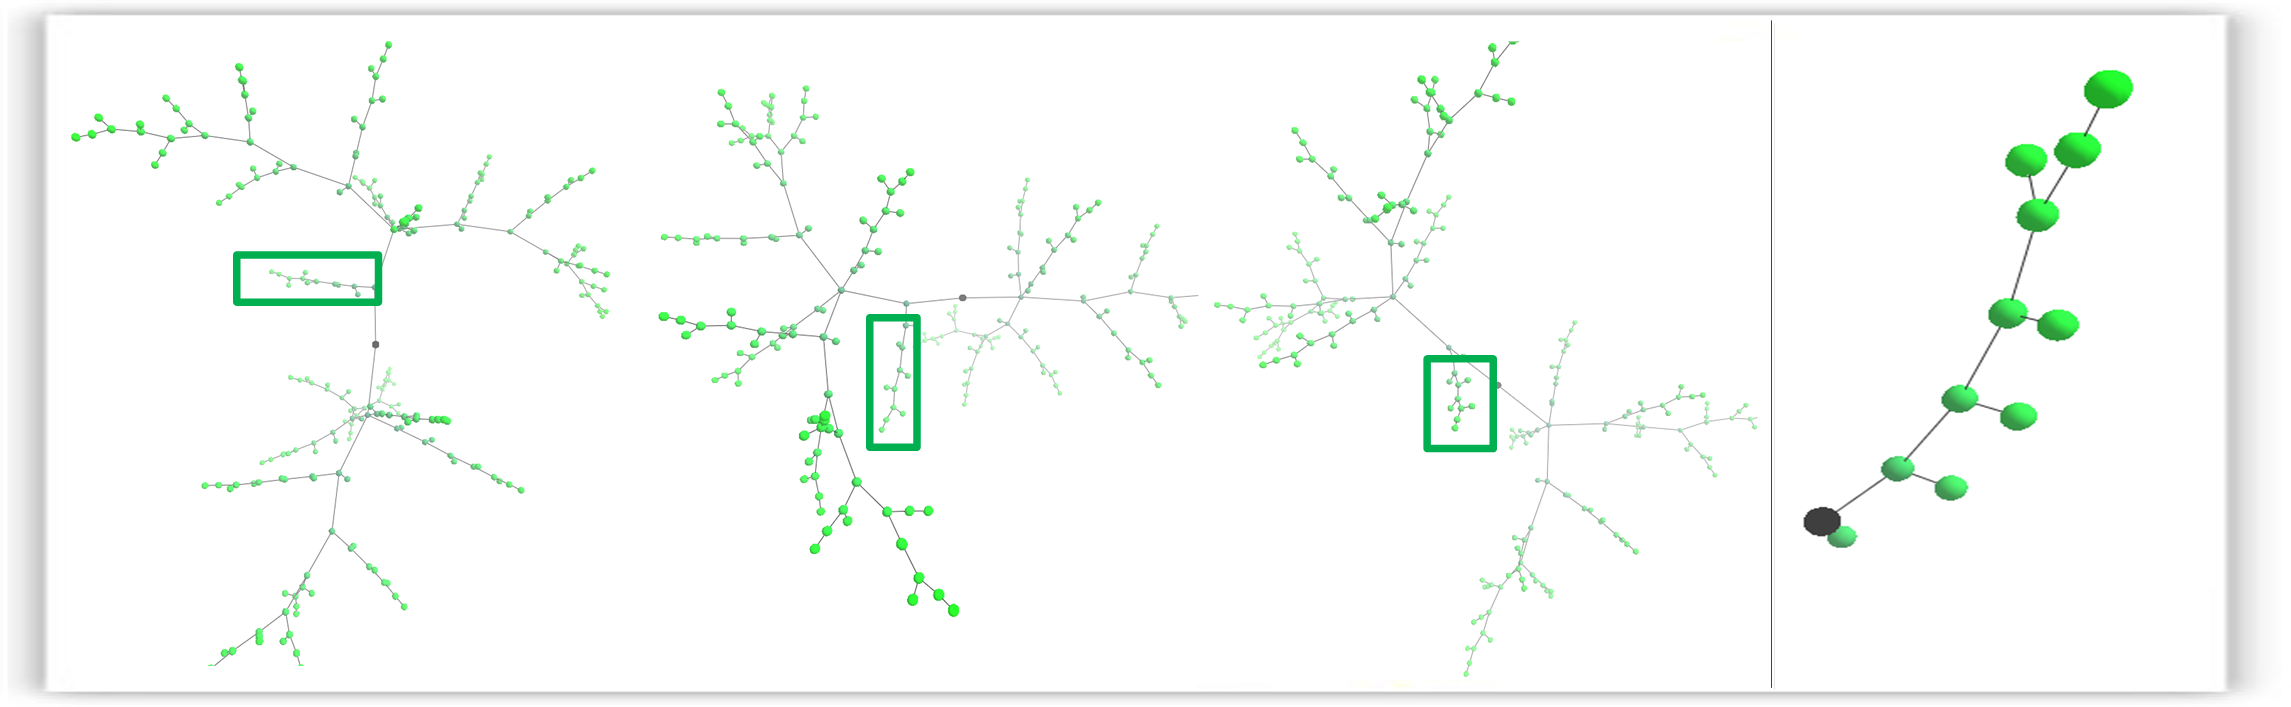
\includegraphics[width=10cm]{Img/phi_prooftreegraph_angles.png}
	\caption{从不同角度观察图形}
	\label{vmdv:prooftree:different:angle}
\end{figure}
\paragraph{图形选中与高亮}
通常在一个3D图形中,在需要呈现局部信息(比如公式的结构、Kripke模型中的状态等)时,我们需要用鼠标来选中,从而高亮某个节点,这时就可以观察被选中的节点的详细信息。\tool{VMDV}中的选中与高亮是可在不同的图形中同步进行的,比如当高亮一棵\sctlprov{}的证明树上的节点时,这个节点对应的公式的相关状态也会在显示Kripke模型的图形中高亮出来。 在\tool{VMDV}中,选中节点的操作既可以通过鼠标左键在节点上点击,也可以通过键盘搜索满足相应条件的节点 (如图\ref{vmdv:prooftree:high:different})。
\begin{figure}[h!]
	\centering
	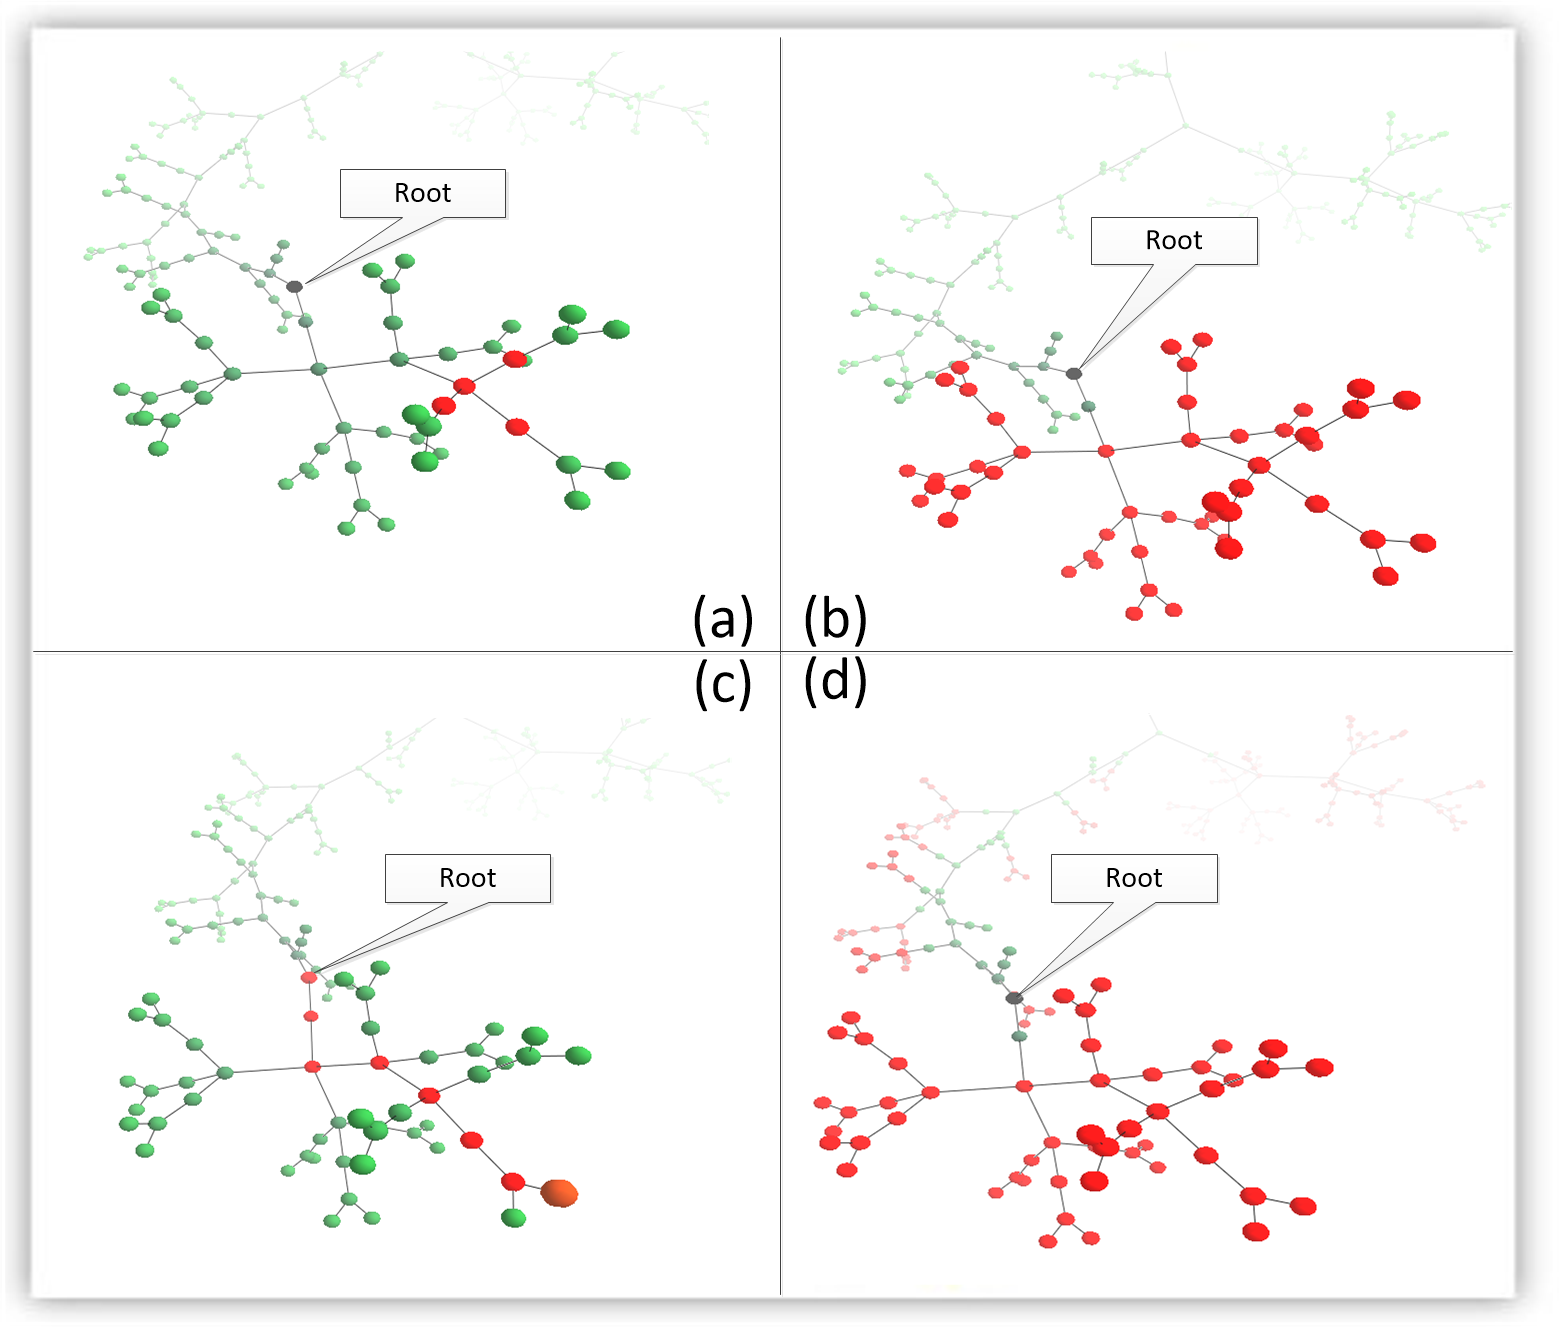
\includegraphics[width=10cm]{Img/high_different.png}
	\caption{高亮图形的不同部分:(a) 高亮单个节点及其后继;(b) 高亮一棵子树;(c) 高亮一个节点的所有祖先;(d) 高亮所有同一类型的公式的子证明}
	\label{vmdv:prooftree:high:different}
\end{figure}
\paragraph{触发自定义操作}
除了以上介绍的用户操作之外,\tool{VMDV}还提供了一种功能来实现对图形的自定义操作。由于\tool{VMDV}可与不同的定理证明工具适配,因此,在一些常用操作之外,\tool{VMDV}中还应该定义一些与特定的定理证明工具相关的操作,比如在\sctlprov{}中,当高亮证明树上的节点时,状态图上的节点也随之自动高亮;在\tool{Coq}中,当选中证明树上的某个节点时,用户可自行选择是否继续证明该节点上的公式。
在\tool{VMDV}中实现自定义操作的方式分为两步:第一步,详细定义自定义操作的方式,即对图形的操作;第二步,定义触发自定义操作的方式。在第一步中,我们利用Java语言的面向对象的特性,首先定义一个\code{AssistAffect}抽象类,然后将所有的对图形的操作均包装成\code{AssistAffect}的子类,这样在程序的编译过程中编译器不需要知道图形的操作的细节,而是在运行时按需调用相应的\code{AssistAffect}子类。由此,我们实现了主程序代码与自定义的图形操作代码的分离。在第二步中,我们同样将触发自定义操作的代码与主程序代码分离开来,具体做法是将触发自定义操作的代码定义为实现\tool{Java}接口\code{PopupItem}的类,由类的继承关系可知,所有实现接口\code{PopupItem}的类均可视为弹出菜单项,且可在窗口中通过鼠标右键触发。因此,当点击由鼠标右键触发的弹出菜单项时,相应的自定义操作即可执行(如图\ref{vmdv:prooftree:userdefined})。
\begin{figure}[h!]
	\centering
	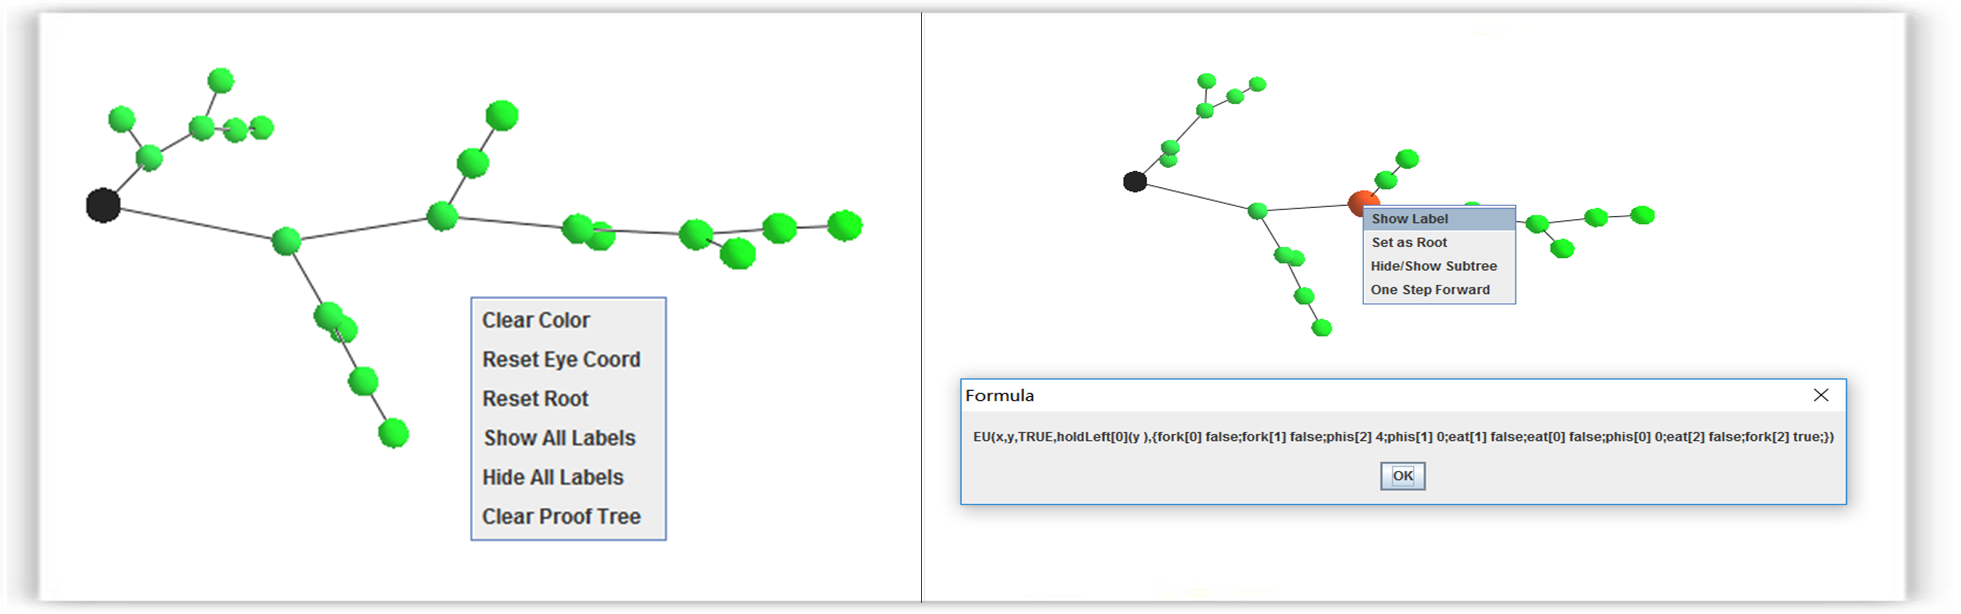
\includegraphics[width=10cm]{Img/user_defined_operation}
	\caption{\tool{VMDV}中的自定义操作}
	\label{vmdv:prooftree:userdefined}
\end{figure}
\paragraph{节点搜索}
在\tool{VMDV}中,虽然节点可通过鼠标逐个高亮显示,但这种方式往往效率过低。为了解决这个问题,我们在\tool{VMDV}中增加了节点搜索的功能以实现节点的批量高亮显示。\tool{VMDV}中的节点搜索是通过将每个节点的标签(即所代表的公式的字符串表示)与输入的正则表达式\footnote{\url{https://en.wikipedia.org/wiki/Regular_expression}}进行匹配,然后将匹配成功的节点高亮显示出来。
(如图\ref{vmdv:prooftree:search})。
\begin{figure}
	\centering
	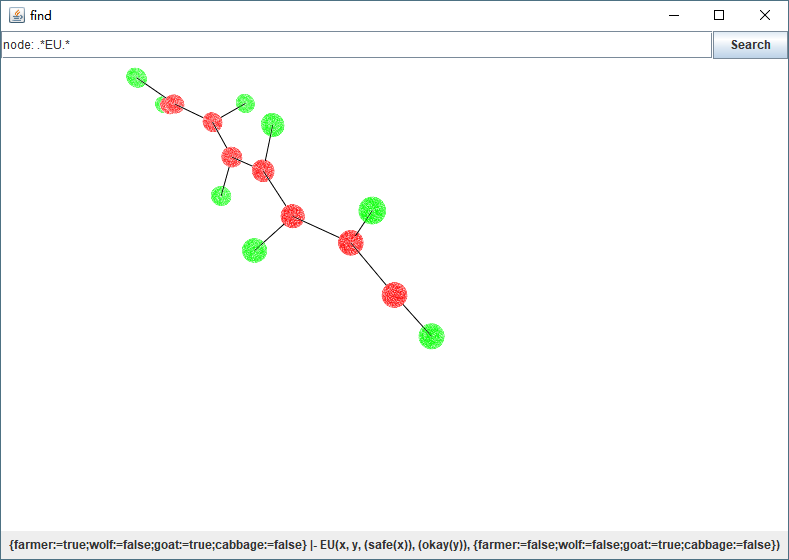
\includegraphics[width=10cm]{Img/vmdv_search.png}
	\caption{\tool{VMDV}中搜索节点}
	\label{vmdv:prooftree:search}
\end{figure}

\subsection{\tool{VMDV}中3D图形的动态布局算法}
在3D图形的可视化系统中,布局算法的作用是计算图形的每个部分在3D空间坐标系中的坐标使得图形的每个部分尽量减少重叠。
由于\tool{VMDV}中图形的所有节点均可动态添加或删除,因此\tool{VMDV}的布局算法必须是连续的,即算法是连续运行、随时更新的。
而且,同样由于\tool{VMDV}的图形具有动态更新的特性,图形中的所有部分必须用同一种方式显示,比如所有的节点统一显示为实心球,所有的边统一显示为实线。同样,为了保持图形显示的统一性,图形的布局算法也必须是统一的,即图形的每个部分用同一种方式布局。
\tool{VMDV}中的布局算法基于ForceAtlas2算法\cite{jacomy2014forceatlas2},该算法同时满足了\tool{VMDV}对布局算法连续性和统一性的要求。类似的布局算法还有OpenOrd算法\cite{martin2011openord}以及Yifan Hu算法\cite{yifanhu05}。不同于ForceAtlas2算法,OpenOrd算法既不是连续的也不是统一的,而Yifan Hu算法是统一的,但不是连续的。与ForceAtlas2算法一样,\tool{VMDV}中的布局算法的基本原理为:首先,图形中每个部分的坐标是根据其受力的大小而变化的,其中每对节点之间具有斥力,力的大小与节点间距离的大小成反比,同时每对以边相连的节点之间具有相互的引力,引力大小与边的长度成正比;然后,当根据每个节点的受力情况更新完其坐标后,再根据新的坐标计算其在新位置上的受力,直至达到受力平衡状态。

\section{\tool{VMDV}的应用}
在本小节中,我们首先考虑\tool{VMDV}在定理证明工具\sctlprov{}的一个应用:可视化证明树和Kripke模型,然后,我们介绍如何将\tool{VMDV}应用在定理证明工具\tool{Coq}中。
\paragraph{\tool{VMDV}在定理证明工具\sctlprov{}的一个应用}
\begin{example} [过河问题]
	一位农夫带着一头狼,一只羊和一筐白菜准备过河,河边有一条小船,农夫划船每次只能载狼、羊、白菜三者中的一个过河。农夫不在旁边时,狼会吃羊,羊会吃白菜。问农夫该如何过河。
\end{example}	
	过河问题可以被描述为一个模型检测问题:假设农夫准备带着狼、养、白菜从河岸A到达河岸B,Kripke模型中的每个状态由四个布尔类型的状态变量{$farmer$}、$wolf$、$goat$以及$cabbage$组成,分别代表农夫、狼、羊以及白菜在河岸A或者河岸B。,那么对于一个状态$s$,如果$farmer$的赋值为$true$,那么代表在状态$s$中农夫在河岸B,其他状态变量的赋值以此类推。因此,Kripke模型中的初始状态为:$$s_0=\{farmer := false, wolf := false, goat := false, cabbage := false\}$$
	Kripke模型中的迁移则表示为农夫在过河过程中所有的状态变量的赋值的变化。该模型检测问题则可表述为是否存在一个由$s_0$可达的状态$s$使得
	$$s=\{farmer := true, wolf := true, goat := true, cabbage := true\}$$
	而且在从$s_0$到$s$的路径上的所有的状态$s'$上,狼不能单独和羊在一起,且羊不能单独和白菜在一起。
	该模型检测问题可用\CTLP{}公式表示为:$$EU_{x,y}(safe(x), complete(y))(s_0)$$
	其中$safe(x)$表示在状态$x$中狼不能单独和羊在一起,且羊不能单独和白菜在一起,而$complete(y)$表示在状态$y$中农夫、狼、羊以及白菜均安全到达河岸B。
	
	利用\tool{VMDV},我们可以将\sctlprov{}对该问题的验证过程进行可视化(见图\ref{vmdv:river:step}),其中上述\CTLP{}公式的证明树在\tool{VMDV}中逐步显示出来,而且随着证明树的逐步显示(图\ref{vmdv:river:step}上半部分),该问题的Kripke模型也逐步构造出来(图\ref{vmdv:river:step}下半部分)。当证明构造完成之后,且将所有的对应于带有$EU$模态词的公式的节点进行高亮显示时,在状态图中则对应着一个路径的高亮显示,该路径即为从$s_0$到$s$的路径,即农夫、狼、羊以及白菜均安全从河岸A到达河岸B的过程(见图\ref{vmdv:river:path})。
	
	\begin{figure}[h!]
		\centering
		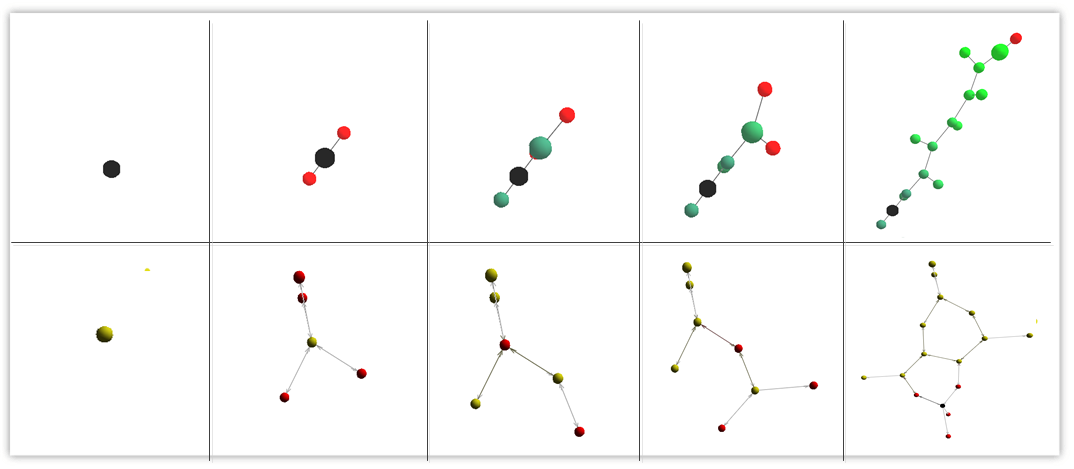
\includegraphics[width=10cm]{Img/river_prooftreegraph_step.png}
		\caption{过河问题的验证过程}
		\label{vmdv:river:step}
	\end{figure}
	\begin{figure}[h!]
		\centering
		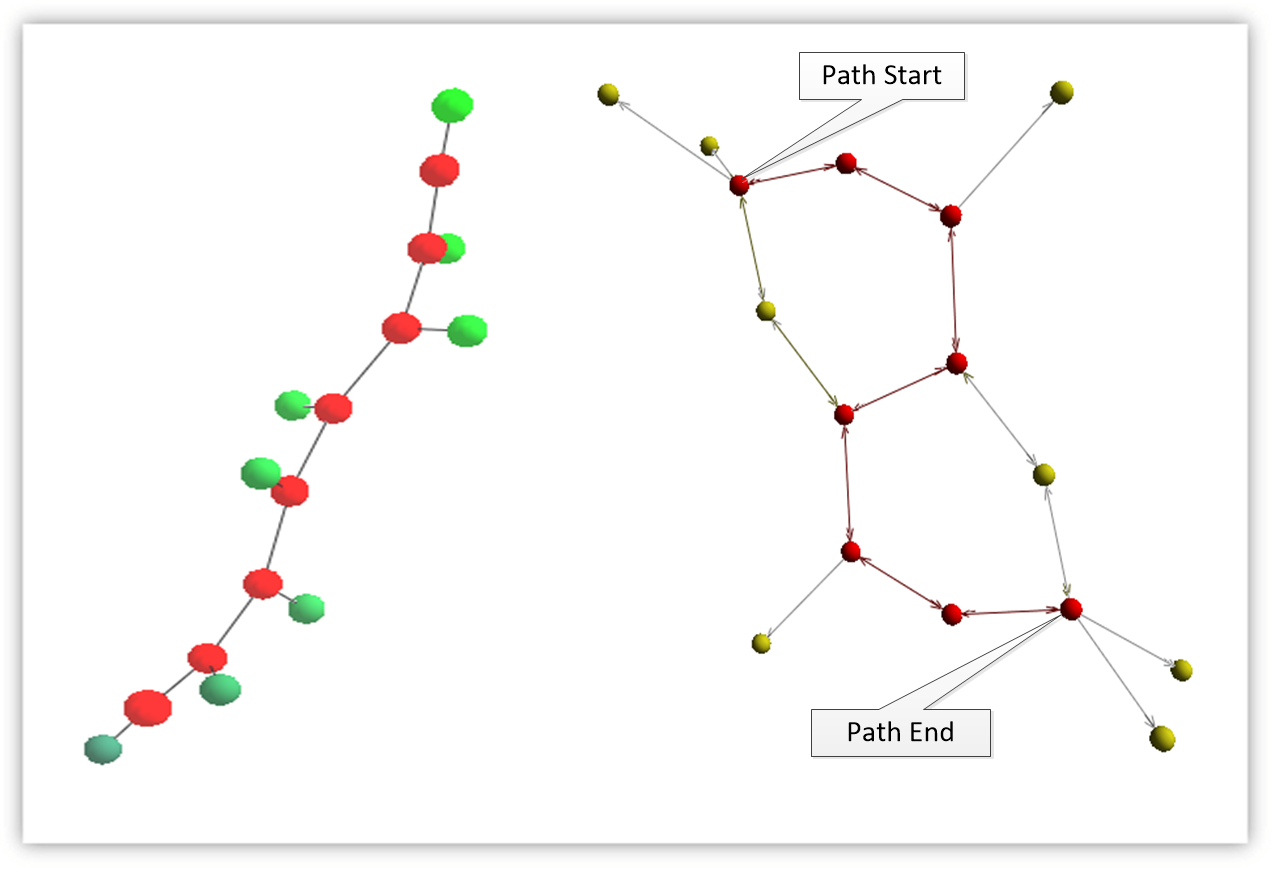
\includegraphics[width=10cm]{Img/river_prooftreegraph_state_highlight.png}
		\caption{过河问题中证明树和状态图的高亮显示}
		\label{vmdv:river:path}
	\end{figure}

	需要注意的是,在\sctlprov{}中,在对不同公式的验证过程中,需要访问的状态个数也往往不同,比如在上述过河问题中,对$EU$公式的验证意味着需要在Kripke模型中寻找一条满足特定条件的路径的过程,因此当对$EU$公式的验证结束并成功之后,相应的状态图中只包含该路径上的节点及其后继。然而,当验证非$EU$的公式,比如$AG$公式时,如果要验证的公式成立,那么\sctlprov{}往往需要访问Kripke模型的所有状态,这时状态图也会相对更大(见图\ref{vmdv:example:ag}),此时,由于$AG$公式的证明树及其状态图往往很大,我们可以利用\tool{VMDV}的局部选中功能,每次观察证明树的时候只观察选中的部分,相应的状态图中也只高亮显示相关的节点(见图\ref{vmdv:example:ag:part})。
	\begin{figure}[h!]
		\centering
		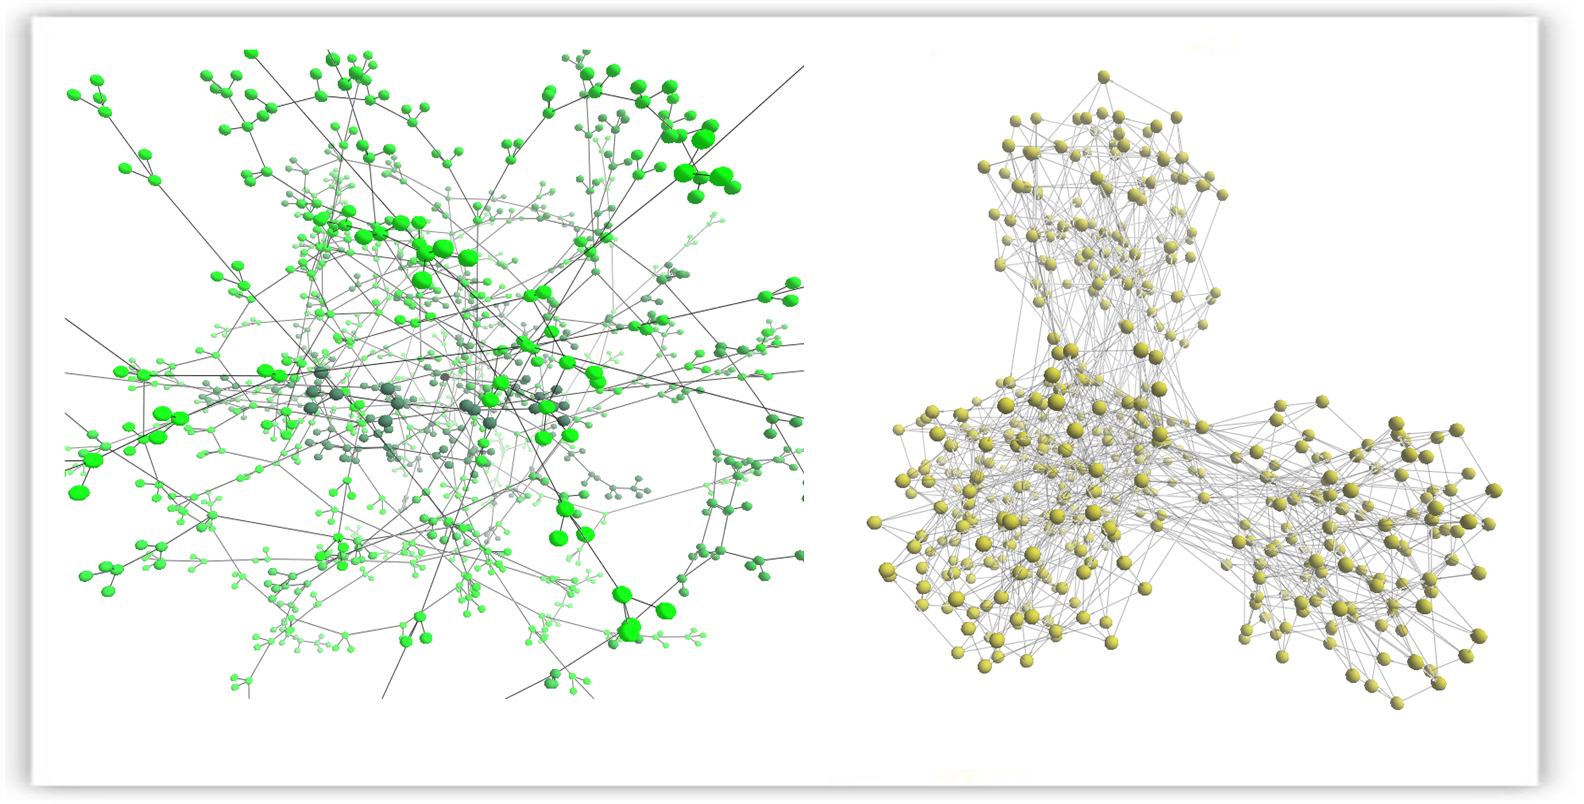
\includegraphics[width=10cm]{Img/ag_proof_state.png}
		\caption{一个$AG$公式的证明树及其状态图}
		\label{vmdv:example:ag}
	\end{figure}
	\begin{figure}[h!]
		\centering
		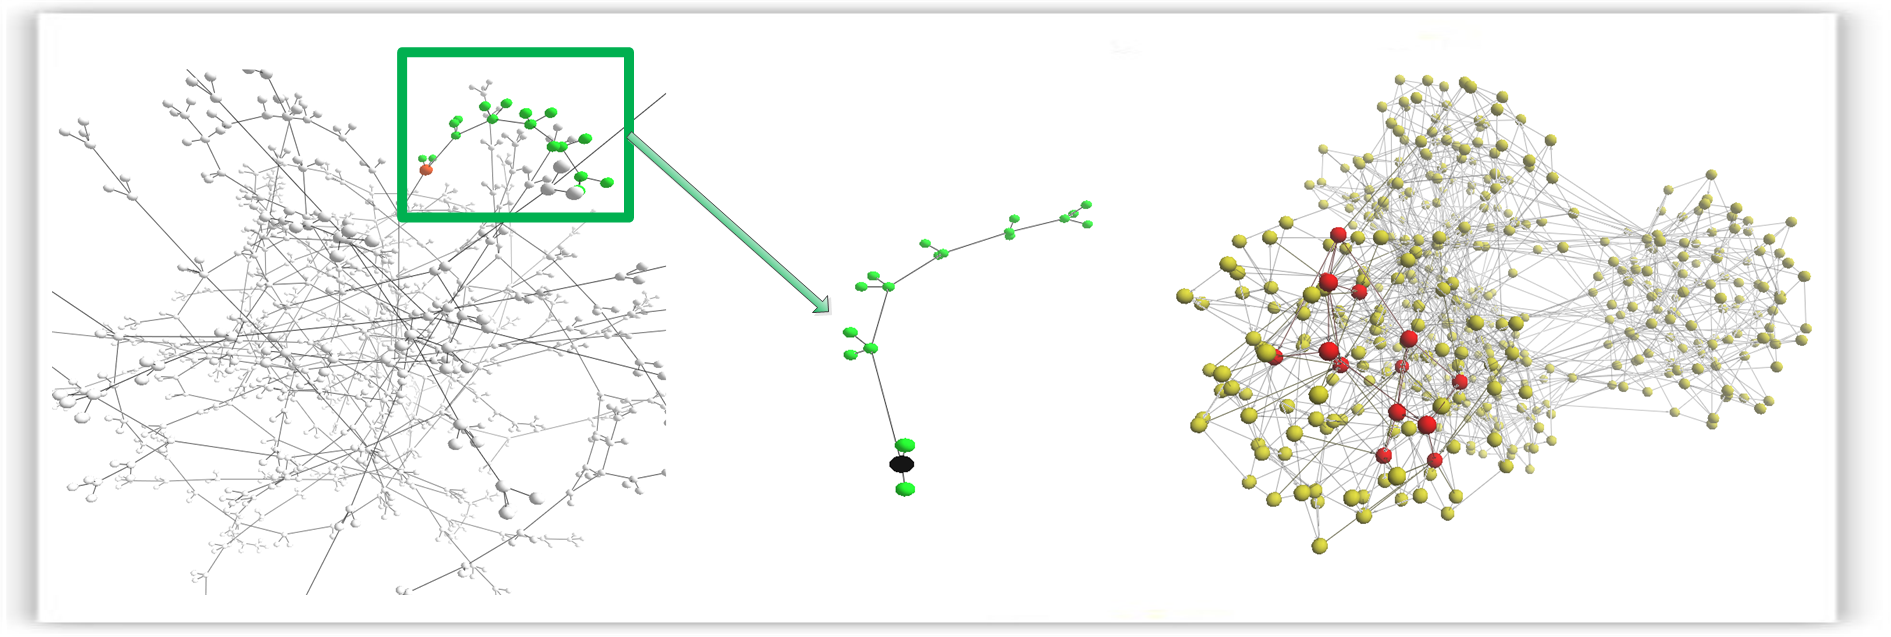
\includegraphics[width=10cm]{Img/ag_part_detail.png}
		\caption{证明树的部分选中以及状态图的部分高亮}
		\label{vmdv:example:ag:part}
	\end{figure}
\paragraph{\tool{VMDV}与定理证明工具\tool{Coq}的结合}
与\sctlprov{}不同,\tool{Coq}中的证明树不是自动生成的,而是由编程人员通过输入证明脚本(Proof Script)来人工干预证明树的产生过程,其中每个证明脚本又包含若干条证明语句。在\tool{Coq}中,每个需要证明的公式被称为一个目标,而该公式的所有前提则被称为该目标的子目标。一个目标的子目标是通过一条证明语句而生成的。
因此,\tool{Coq}的证明树可表示为:将每个公式(目标)都看成证明树中的节点,而且将该公式的前提(子目标)看成相应的节点的后继,如果该公式没有前提,则其对应的节点为叶节点。
为了将\tool{Coq}中的证明树在\tool{VMDV}中可视化,我们开发了一个用于协调\tool{VMDV}与\tool{Coq}之间通信的中间件\tool{Coqv}\footnote{\url{https://github.com/terminatorlxj/coqv}}:\tool{Coqv}与\tool{Coq}的通信遵循\tool{Coq}自定义的XML通讯协议\footnote{\url{https://github.com/siegebell/vscoq/wiki/XML-protocol}};\tool{Coqv}与\tool{VMDV}的通信遵循\tool{VMDV}的JSON通讯协议。通过\tool{Coqv},\tool{VMDV}可实现对\tool{Coq}中生成的证明树的可视化。
例如,公式$$\forall A B C: Prop, (A\rightarrow(B\rightarrow C)\rightarrow ((A\rightarrow B)\rightarrow(A\rightarrow C)))$$的证明脚本如下。
\begin{center}
%	\centering
%	\begin{tabular}{p{5cm}}
		\begin{verbatim}
		Proof.
		    intros A B C.
		    intros H1 H2 H3.
		    apply H1. assumption.
		    apply H2. assumption.
		Qed.
		\end{verbatim}
%	\end{tabular}
	
%	\caption{一个公式在\tool{Coq}中的证明脚本}
%	\label{vmdv:coq:proofscript}
\end{center}
该证明脚本所生成的证明树在\tool{VMDV}中可视化如图\ref{vmdv:coq:vis}所示。图中证明树的生成分别由6步完成,分别对应于证明脚本的6个命令。
\begin{figure}[h!]
	\centering
	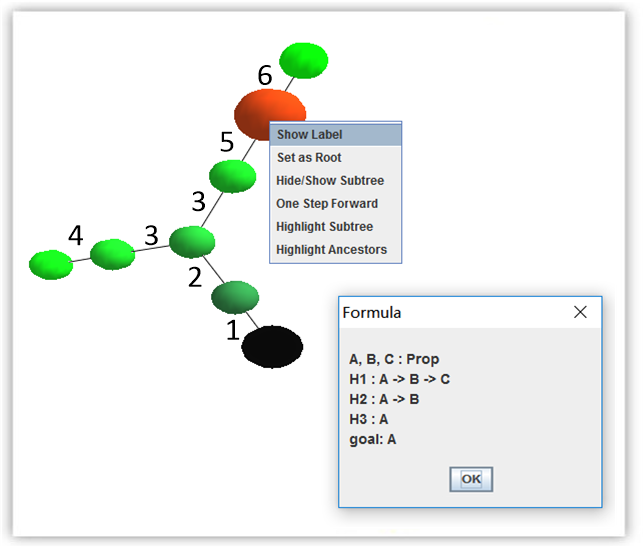
\includegraphics[width=7cm]{Img/coq_example.png}
	\caption{\tool{Coq}中的一棵证明树的可视化}
	\label{vmdv:coq:vis}
\end{figure}
目前,\tool{Coqv}的开发阶段已完成,目前正在根据\tool{Coq}的不同应用场景进行测试,并逐步完善功能,这也是本论文的其中一项未来工作。

\section{本章小节}
本章的内容介绍的是证明可视化工具\tool{VMDV}。起初,\tool{VMDV}的提出是为了解决上一章提出的定理证明工具\sctlprov{}的可视化问题:通过以3D图形的方式展示\sctlprov{}输出的证明树来达到理解输出结果并优化建模方式的目的。不过,为了一般性起见,我们将\tool{VMDV}设计成了可以匹配不同的定理证明工具的可视化系统:定理证明工具(或其插件)通过实现\tool{VMDV}预先定义的通讯协议来达到与\tool{VMDV}进行交互并可视化的目的。不同于现有的证明可视化工具,\tool{VMDV}的图形显示效果更好,而且其动态布局算法能更好的适应交互式定理证明的可视化。
